\documentclass{scrarticle}
\usepackage[utf8]{inputenc}
\usepackage{graphicx}
\usepackage{float}
\usepackage[T1]{fontenc}
\usepackage{listings}

\title{SpaceWalk The Game}
\author{Péter Bence, Vasánszki Milán, Székely Katalin, Tóth Balázs\\A Foobar Reloaded csapata\\Modern szoftverfejlesztési eszközök\\GKNB\_INTM006}
\date{October 2022}

\begin{document}

\maketitle
\begin{figure}[H]\centering
    
\includegraphics[width=0.4\columnwidth]{sze_logo.png}\label{fig:logo}
\end{figure}
\newpage
\tableofcontents
\newpage

\section{Alapinformációk} 
Ez a specifikáció egy szöveges, szerepjátékos űrkalandjátékhoz készült. A játék- ban mozoghatsz szobáról szobára, gyűjthetsz tárgyakat és új utakat nyithatsz meg a játék világának felfedezéséhez. Találkozhatsz és interakcióba léphetsz NPC-kkel. A program a felhasználótól vár egyszerűbb parancsokat, amelyeket később eseményként megjelenít. A történet 20 mélységű. Az alkalmazás a felhasználó által adott helytelen bemenetre hibaüzenettel válaszol.

\section{Történetvázlat}
Az év 2094. A mesterséges intelligencia teljes mértékben átvette az irányítást a Föld nevezetű bolygó felett 30 évvel ezelőtt. De nem úgy ahogy gondolod kedves PLAYERNAME. 2064-ben kifejlesztették az Oázis AI-t, ami egyedül azt a cél szolgálja, hogy az emberek kényelemben éljenek. A tökéletes utópisztikus világ, ahol az emberek azért jönnek a Földre, hogy jól érezzék magukat, azzal foglalkozzanak, amivel csak akarnak, és akkor, amikor akarnak. Minden unalmas és monoton feladat elvégzését átvették a robotok és az OAI. Ebbe beletartozik a teljesen automatizált házvezetés, takarítás, bevásárlás, és még a főzés is. Nem kevés következménnyel járt ez az átállás. Beolvasztották az összes fegyvert, megszüntették az autókat, és csak is mindenki buszokkal, vagy kijelölt szállítási eszközzel közlekedhet. A 2045-ös jégkorszak után nagymértékben megcsappant a Föld lakossága. A tervezett 9,44 milliárd ember helyett kevesebb, mint 1 milliárd maradt. Itt kezdődik a napod. Ma van a huszonötödik születésnapod, és nagy terveid vannak a mai napra. Megnyitott az első űr bár és szálló, amit pár nappal ezelőtt állítottak Föld körüli pályára, és benne vagy a szerencsés 100 ember között, akik részt vehetnek a megnyitó rendezvényen. A SpaceWalk™ nevezetű bár óriási hírnévnek örvend. Több tíz éve beszélnek róla, hogy folyamatosan építik, részről részre szobáról szobára. Most ért véget az építkezés, és mindenki részt akar venni a megnyitón. Nagyon sok feltételnek meg kellett felelni, és ezen kívül egy pályázatot is be kellett adni, hogy miért te legyél a kiválasztott, aki részt vehet ezen a rendezvényen. Az, hogy izgatott vagy az egy enyhe alábecslés. Miket is ígér a SpaceWalk™? Kezdésnek egy űrsétával kezdődik az este, ami a legelső dolog, miután megérkezel az űrállomáshoz. Ezek után svédasztalos vacsora, korlátlan bár fogyasztás, diszkó, és az éjszaka végén kényelmes ágyak várják a vendégeket a hotel szobákban.  Az este nagyon jól telt, viszont az éjszaka folyamán, rázkódásra ébredsz, és nem tudod mi történik. Vajon egy aszteroida találhatta el az állomást? Vagy valami meghibásodás állhat a háttérben? Lehet szabotázs? Elképzelhető, hogy ennél sokkal sötétebb történések állhatnak a háttérben? Derítsük ki!

\section{Követelmények}
\begin{table}[H] \centering
    \caption{Követelmények}\label{tab:requirements}
    \begin{tabular}{@{}ll@{}}
        \emph{Eset} & \emph{Leiras}\\ \hline
        1. Szobarendszer & A játék világának a felépítése, szobákból álljon.\\
        2. Mozgás & A játékos tudjon mozogni szobárol szobára.\\
        3. Környezeti interakció & A játékos tudjon interakcióba lépni környezetével.\\ & Szobák átkutatása, tárgyak megvizsgálása és felvétele,\\ & a játékban élő NPC-kel való interakció.\\
        4. Történet vonalának követése & Küldetéseken keresztül tudjon a játékos a sztorival haladni.\\
    \end{tabular}
\end{table}

\section{Használati esetek}
\begin{table}[H] \centering
    \caption{Használati esetek}\label{tab:usecasetable}
    \begin{tabular}{@{}ll@{}}
        \emph{Eset} & \emph{Leiras}\\ \hline
        1. Move (player)         & Mozgás szobáról szobára.\\
        2. Search room (player)  & Szoba átkutatása tárgyak és NPC-k után.\\
        3. Pick up item (player) & Talált tárgyak felvétele, megviszgálása.\\
        4. Interact with NPC (player) & Talált NPC-vel való kommunikáció.\\
        5. Accept mission (player) & Talált NPC küldetésének felvétele.\\ 
        6. Unlock Room (game) & Ha a játékosnál van kulcs a szobához,\\ & a játék automatikusan kinyitja azt.\\
        7. Enter Room (game) & Ha a játékos kiválasztotta a mozgás egyik szobárol\\ & a másikra opciót és van nála kulcs,\\ & a játék átlépteti a kiválsztott szobába.\\
        8. Finish Mission (game) & Ha a küldetés feltételei teljesülnek,\\ & akkor a játék automatikusan lezárja a küldetést.\\ 
    \end{tabular}
\end{table}

\graphicspath{{../Planning/}}
\begin{figure}[H]\centering
    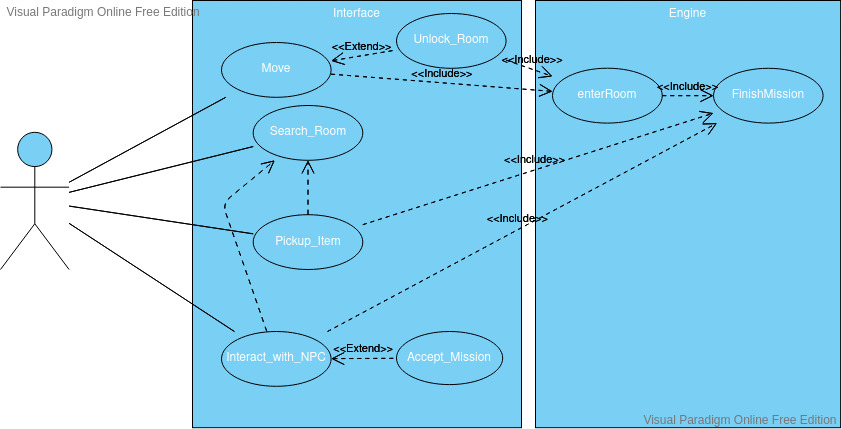
\includegraphics[width=1.0\columnwidth]{Functional_UseCase.jpg}
    \caption{Functional Use Cases}\label{fig:1}
\end{figure}

\section{Struktura}
\begin{figure}[H]
    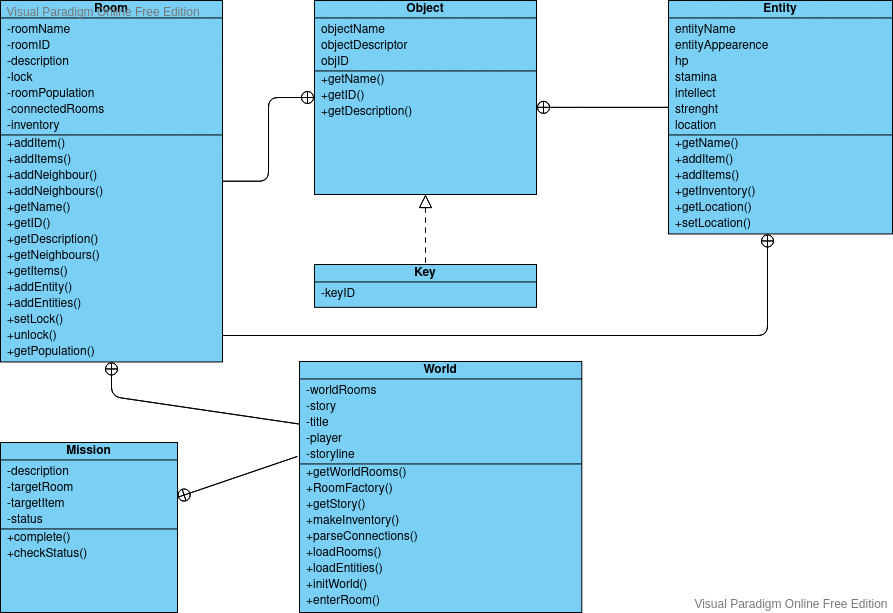
\includegraphics[width=0.75\columnwidth]{Class_Architecture.jpg}
    \caption{Class Architecture}\label{fig:2}
\end{figure}

\subsection{Classok}
\paragraph{class World}
A játék menetét kontrolláló class, a világ környezeti jellemzőit, szobáit, küldetéseit, sztoriát és magát a játékost kezeli. Ez a class fele az világ inicializálásáért, ezt az xml file parsolásával teszi meg.
\paragraph{class Room}
Játék világának fő építőeleme, a szobák kezelik a bennük lévő NPC-ket és tárgyakat.
\paragraph{class Entity}
A világ élőlényeit reprezentáló class, általában a szobákban tárolódnak el, kivéve a játékost reprezentáló Entity objectumot, amit a class World tartalmazza. Mindezek mellett a tárgyak inventoryba mozgazásához szükséges funkciókkal is rendelkezik.
\paragraph{class Object}
Tárgyak reprezentálására használt class.
\paragraph{class Key}
Tárgy class-ból származtatott osztály, ami a szobák nyitási mechanikáját valósítják meg.
\paragraph{class Mission}
A sztori haladásáért felelős osztály, a fő küldetéseket a játék inicializásakor már az aktív küldetések közé helyezzük, az opcionális küldetéseket a szobákban található NPC-től lehet felvenni. A küldetés célját tárolja, a státuszát kezeli és adja vissza és az automatikus befejezését kezeli.

\begin{figure}[H]
    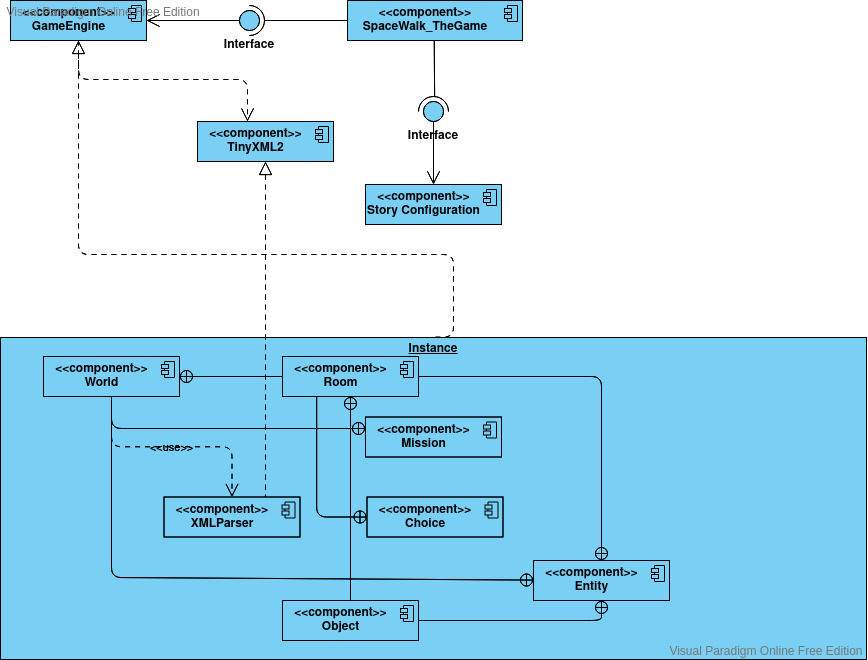
\includegraphics[width=0.75\columnwidth]{Component_Connection.jpg}
    \caption{Component connection}\label{fig:3}
\end{figure}

\paragraph{Engine felépítése}
A játékvilág szobákból tevődik össze, amikben lehet tárgyakkal és NPC-kel interakcióba lépni. Vannak olyan szobák amiket csak kulcsok segítségével lehet kinyitni. A játékvilág felfedezése közben különböző küldetéseket kell végrehajtani, amik a sztori vonalát követik.

\section{Viselkedes}
\begin{figure}[H]
    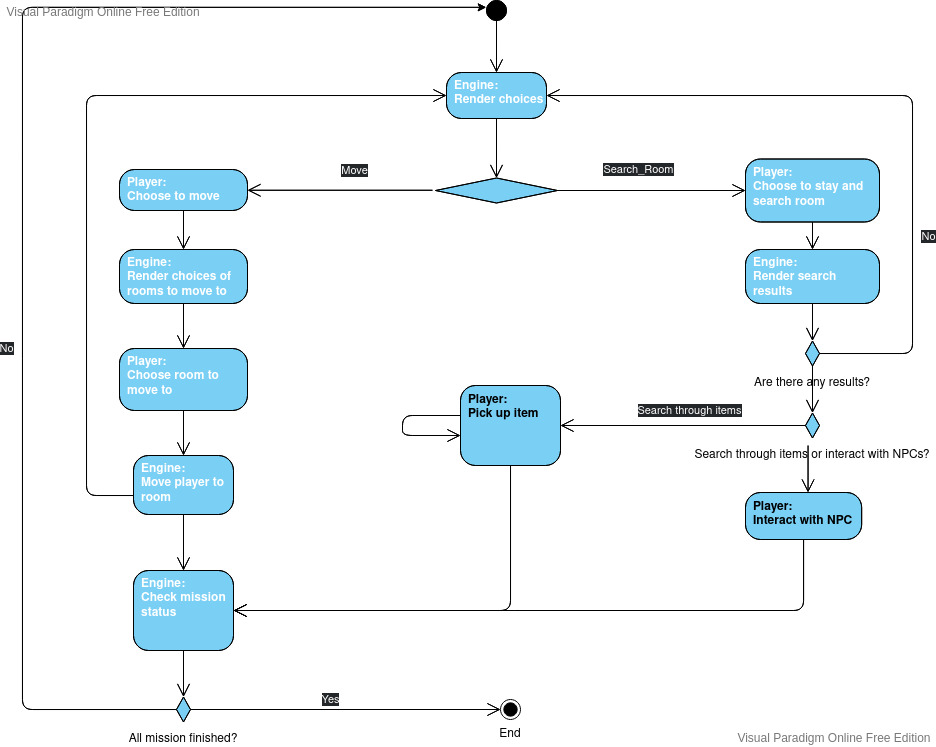
\includegraphics[width=1.0\columnwidth]{GameLoop_ActivityDiagram.jpg}
    \caption{Gameloop Activity Diagram}\label{fig:4}
\end{figure}

\begin{figure}[H]
    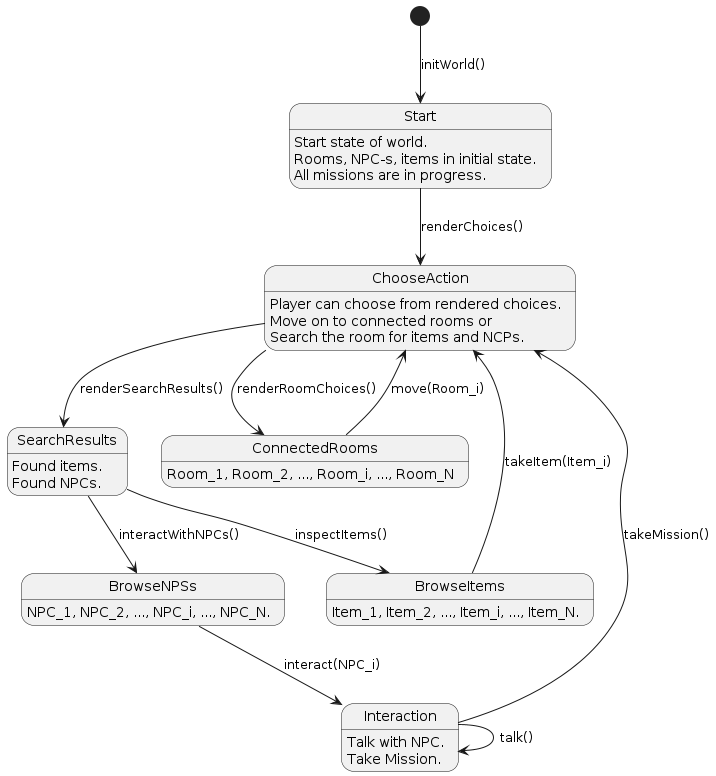
\includegraphics[width=1.0\columnwidth]{State_Machine.png}
    \caption{State Machine}\label{fig:5}
\end{figure}
\newpage

\subsection{Játék menete}
A játék loop jellegűen ajánlja fel a lehetséges tevékenységeket a játékos számára, a tevékenységek ismételten való elvégzésével lehet a küldetések céljait elérni és a sztori vonalán haladni. Lehetséges tevékenységek lehetnek: másik szobába mozgás, szoba átkutatása, tárgy megvizsgálása és felvétele, NPC-vel való interakció, küldetés elfogadása. A tevékenység sorban és egymásból következhetnek. Pl. ha azt választjuk hogy mozogjunk át egy másik szobába, akkor a játék a következő szobában újra felsorolja a lehetséges tevékenységeket, de ha azt választjuk, hogy kutassuk át a szobát, akkor ebből következhenek a tárgyak megvizsgálása vagy NPC-vel való kommunikáció tevékenységek. A küldetések státuszát a játék automatikusan frissíti a játékos tevékenységeinek és döntéseinek alapján.

\section{Történet tárolási formátuma}
A történetet xml fájlformátumban tároljuk és a TinyXML2 könyvtár segítségével olvassuk be. Az xml fájlformátum lehetővé teszi, hogy a játékvilágot és hozzá tartozó történelem részleteket modulárisan építhessük fel, így szabadon bővíthető lesz, vagy akár egy teljesen más történetet is betölthetünk.

\subsection{XML file felépítése}

\subsubsection{<world>}
A <world> tag-ből szigorúan csak egyet szabad használni, mivel ez fogja tartalmazni a játékvilág összes elemét.

\subsubsection{<title>}
<title> tag-ből megint csak egyet szabad használni, ez tartalmazza a játék címét. Ez a tag a <world> tagnek egy gyereke.

\subsubsection{<room>}
A <room> tag segítségével tölthetjük meg szobákkal a világot, ebből a tagből akármennyit lehet használi, de szigorúan a <world> tag-en belül.

\subsubsection{<name>}
A <name> tag a <room> nevét adja meg.

\subsubsection{<description>}
A <description> tag-el lehet a szobának a leírását, szobához tartozó storyt megadni.

\subsubsection{<id>}
Az <id> tag egyértelműen a szoba azonosítója, ami segít az egyszerű azonosításban, a kulcsokkal való összekötéssel és a szomszéd szobák megadásában.

\subsubsection{<inventory>}
A szobában megtalálható tárgyakat foglalja magába az <inventory> tag, amiből szobán-\\ként egy van.

\subsubsection{<object>}
Az <object> tageket az <inventory> tageken belülre kell helyezni, mivel ezzel tudjuk konkrétan megadni egy szobában található tárgynak a tulajdonságait.

\subsubsection{<name>}
Egy tárgynak is van megnevezése, ezért az <object>-en belül is kell használni a name taget.

\subsubsection{<description>}
A tárgyak kinézetét, felhasználási módját a leírás - description - tag-el lehet megadni.

\subsubsection{<id>}
A tárgyakat nehéz lenne csak név és leírás alapján beazonosítani programozási szemszögből így az id tagben megadott id-vel könnyen be lehet azonosítani.

\subsubsection{<entity>}
A szobákban létező NPC-ket az entity tag-el lehet megadni. Az entity-knek is van nevük, a név megadásához az eddig már többször elhangzott <name> tag-el lehet megadni. Az entity-knek is van <inventory>-juk, amiben ugyan úgy lehet megadni a tárgyakat - <object> -, mint a szobáknak.

\subsubsection{<missions>}
Ez az új tag a <world>-tag gyereke, a storyhoz tartózó küldetések megadására szolgál.

\subsubsection{<mission>}
A mission tag-en belül meg kell adni a küldetés leírását <description>-nel adható meg a küldetés leírása. A küldtés célját a <targetRoom> és a <targetItem> tag-el adhatjuk meg, ezeknek a tageknek a szoba vagy tárgy azonosítóját kell tartalmazniuk.

\subsection{Példa az xml story fájl elkészítéséhez}
\lstinputlisting{../test_story.xml}

\newpage
\section{Tesztelés}
\subsection{GoogleTest}
A GoogleTest könyvtár felhasználásával írtunk teszteket amik a tests mappában találhatók. A tesztek magukat a class-okat, a class-ok egymással való komunikációját és a use case-ket fedik le.
\subsection{Példák}
\subsubsection{Room class konstruktorának tesztje}
\begin{lstlisting}
TEST_F(RoomTest, constructor_test) {
    node Room1(
        new Room("Room1", 1, 
                 "This room is created to test the constructor."
        )
    );
    EXPECT_EQ("Room1", Room1->getName());
    EXPECT_EQ(1, Room1->getID());
    EXPECT_EQ("This room is created to test the constructor.", 
              Room1->getDescription()
    );
}
\end{lstlisting}
\subsubsection{Room class item-ekkel való operációja}
\begin{lstlisting}
TEST_F(RoomTest, test_Item_operation_methods) {
    // testItems should have 10 items now
    ASSERT_EQ(10, testItems.size());
    testRooms[0]->addItem(testItems[0]).addItem(testItems[1]);
    // 2 items from testItems were added to testRoom[0]'s 
    // inventory, so now testItems should have 8 items
    ASSERT_EQ(2, testRooms[0]->getItems().size());
    // This unique_ptr should contain a nullptr, 
    // because addItem moved it to the Room's inventory
    EXPECT_EQ(nullptr, testItems[0].get()); 
    EXPECT_EQ(nullptr, testItems[1].get()); // Same as above
    EXPECT_STREQ(std::string("Item No. 0").c_str(), 
                testRooms[0]->getItems()[0]->getName().c_str());
    EXPECT_STREQ(std::string("Item No. 1").c_str(), 
                testRooms[0]->getItems()[1]->getName().c_str());
    }
\end{lstlisting}
\subsection{Github Actions}
A githubnak egy nagyon hasznos funkciója az Actions amivel automatizált Workflow-okat lehet lefuttatni. Mi ennek a funkciónak a segítségével futtatjuk le a megírt teszteket. Ez egy remek újítás, mivel ez megakadályozza a hibás kódok master branchre való feltöltését.
\begin{figure}[H]
    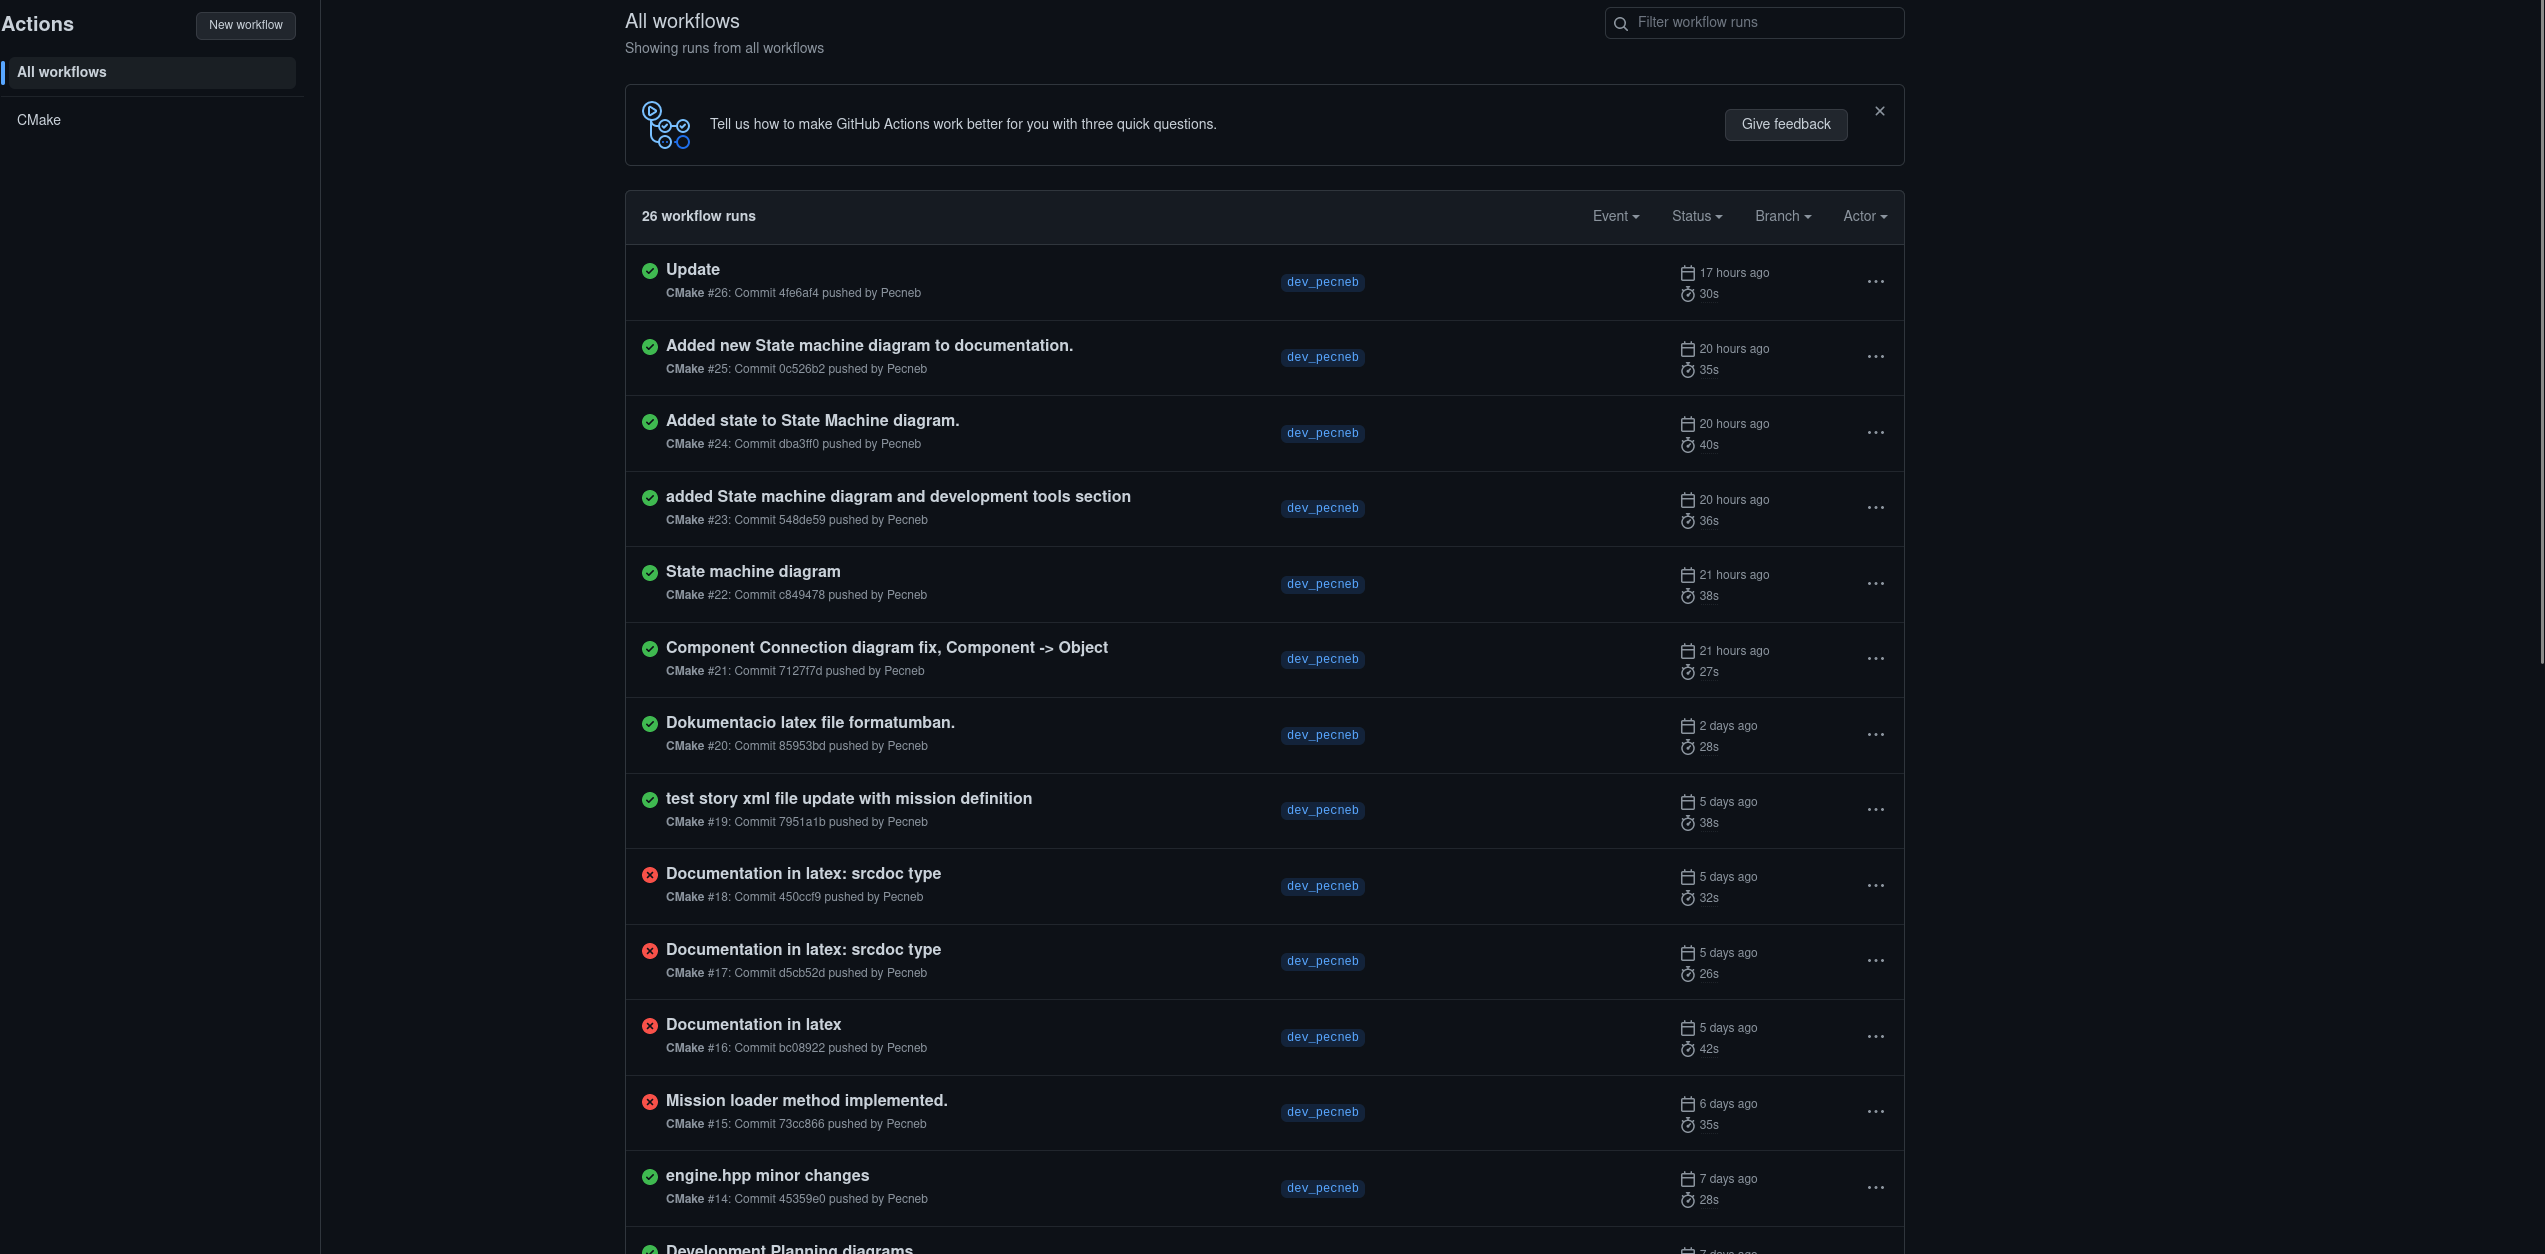
\includegraphics[width=1.0\columnwidth]{github_actions.png}
    \caption{Workflows}\label{fig:6}
\end{figure}
\newpage

\section{Fejlesztés menete}
\subsection{Szoftverfejleszési módszertanok}
A játék fejlesztéséhez scrum és kanban módszertant törekszünk követni. Ehhez a github "Projektek" felülete nyújt segítséget, ahol egy kanban táblán vesszük fel a tevékeny-\\ségeket amik alkotják a backlogot.
\begin{figure}[H]
    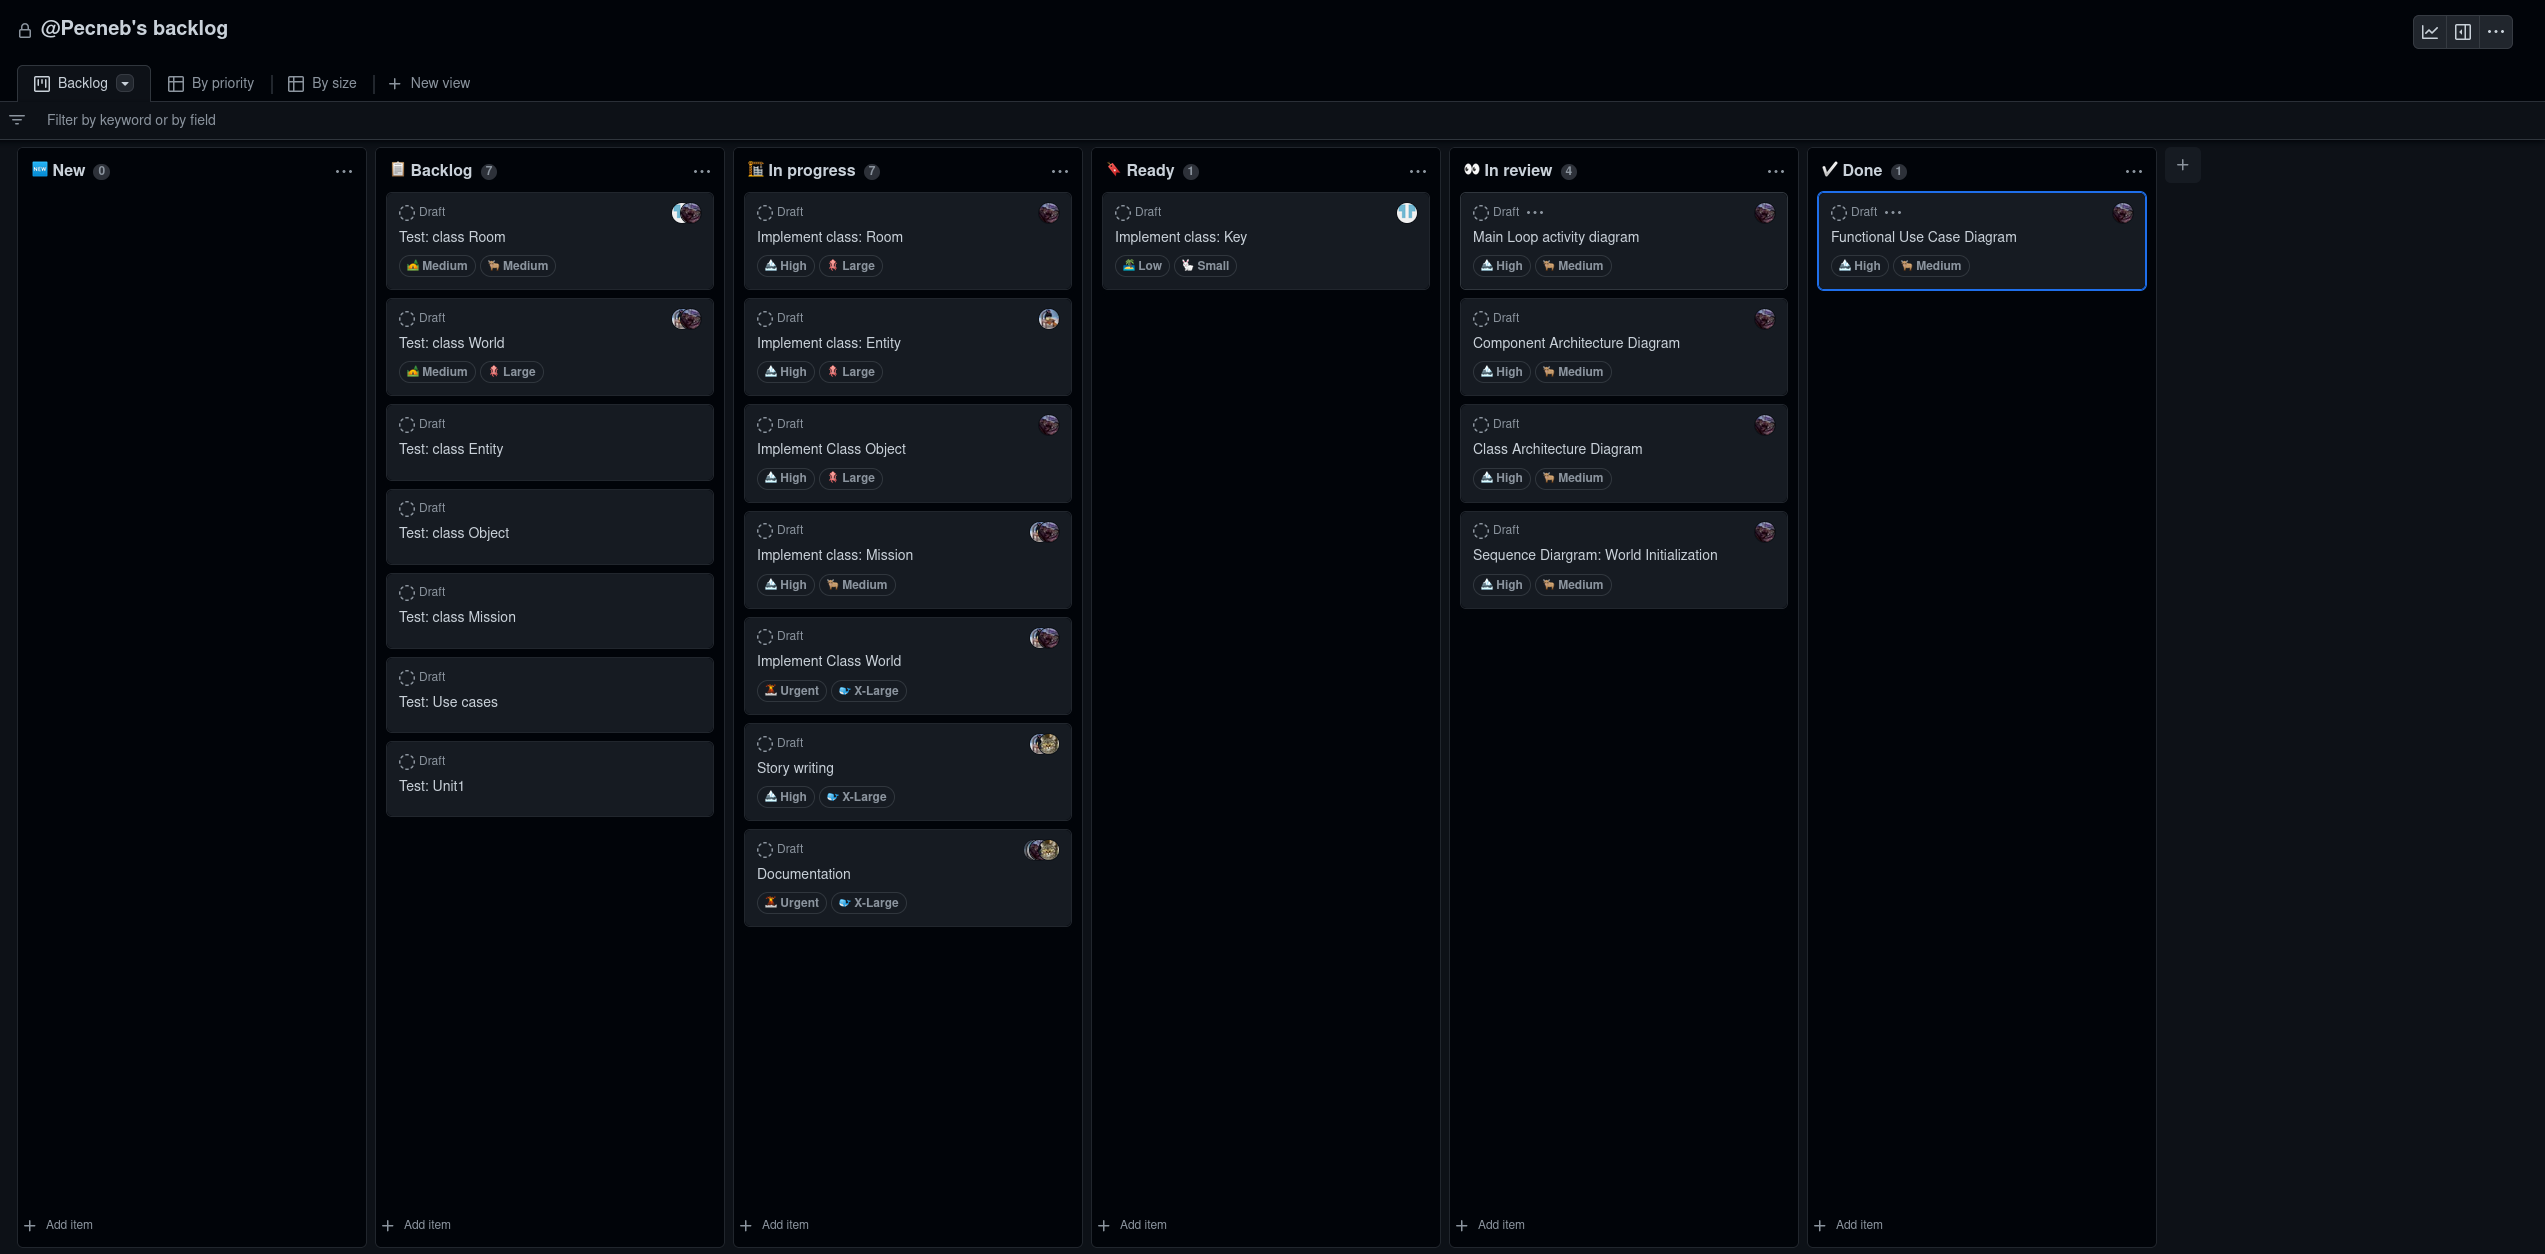
\includegraphics[width=1.0\columnwidth]{kanban_scrum.png}
    \caption{Kanban tábla}\label{fig:7}
\end{figure}
\newpage
\subsection{Dokumentáció}
\subsubsection{Doxygen}
A Doxygen nagy segítségnek bizonyult a fejlesztés során, a kódunk megfelelő kommentelésével hasznos dokumentációt készít számunka, hogy megértsük és fel tudjuk használni a másik kódját.
\begin{figure}[H]
    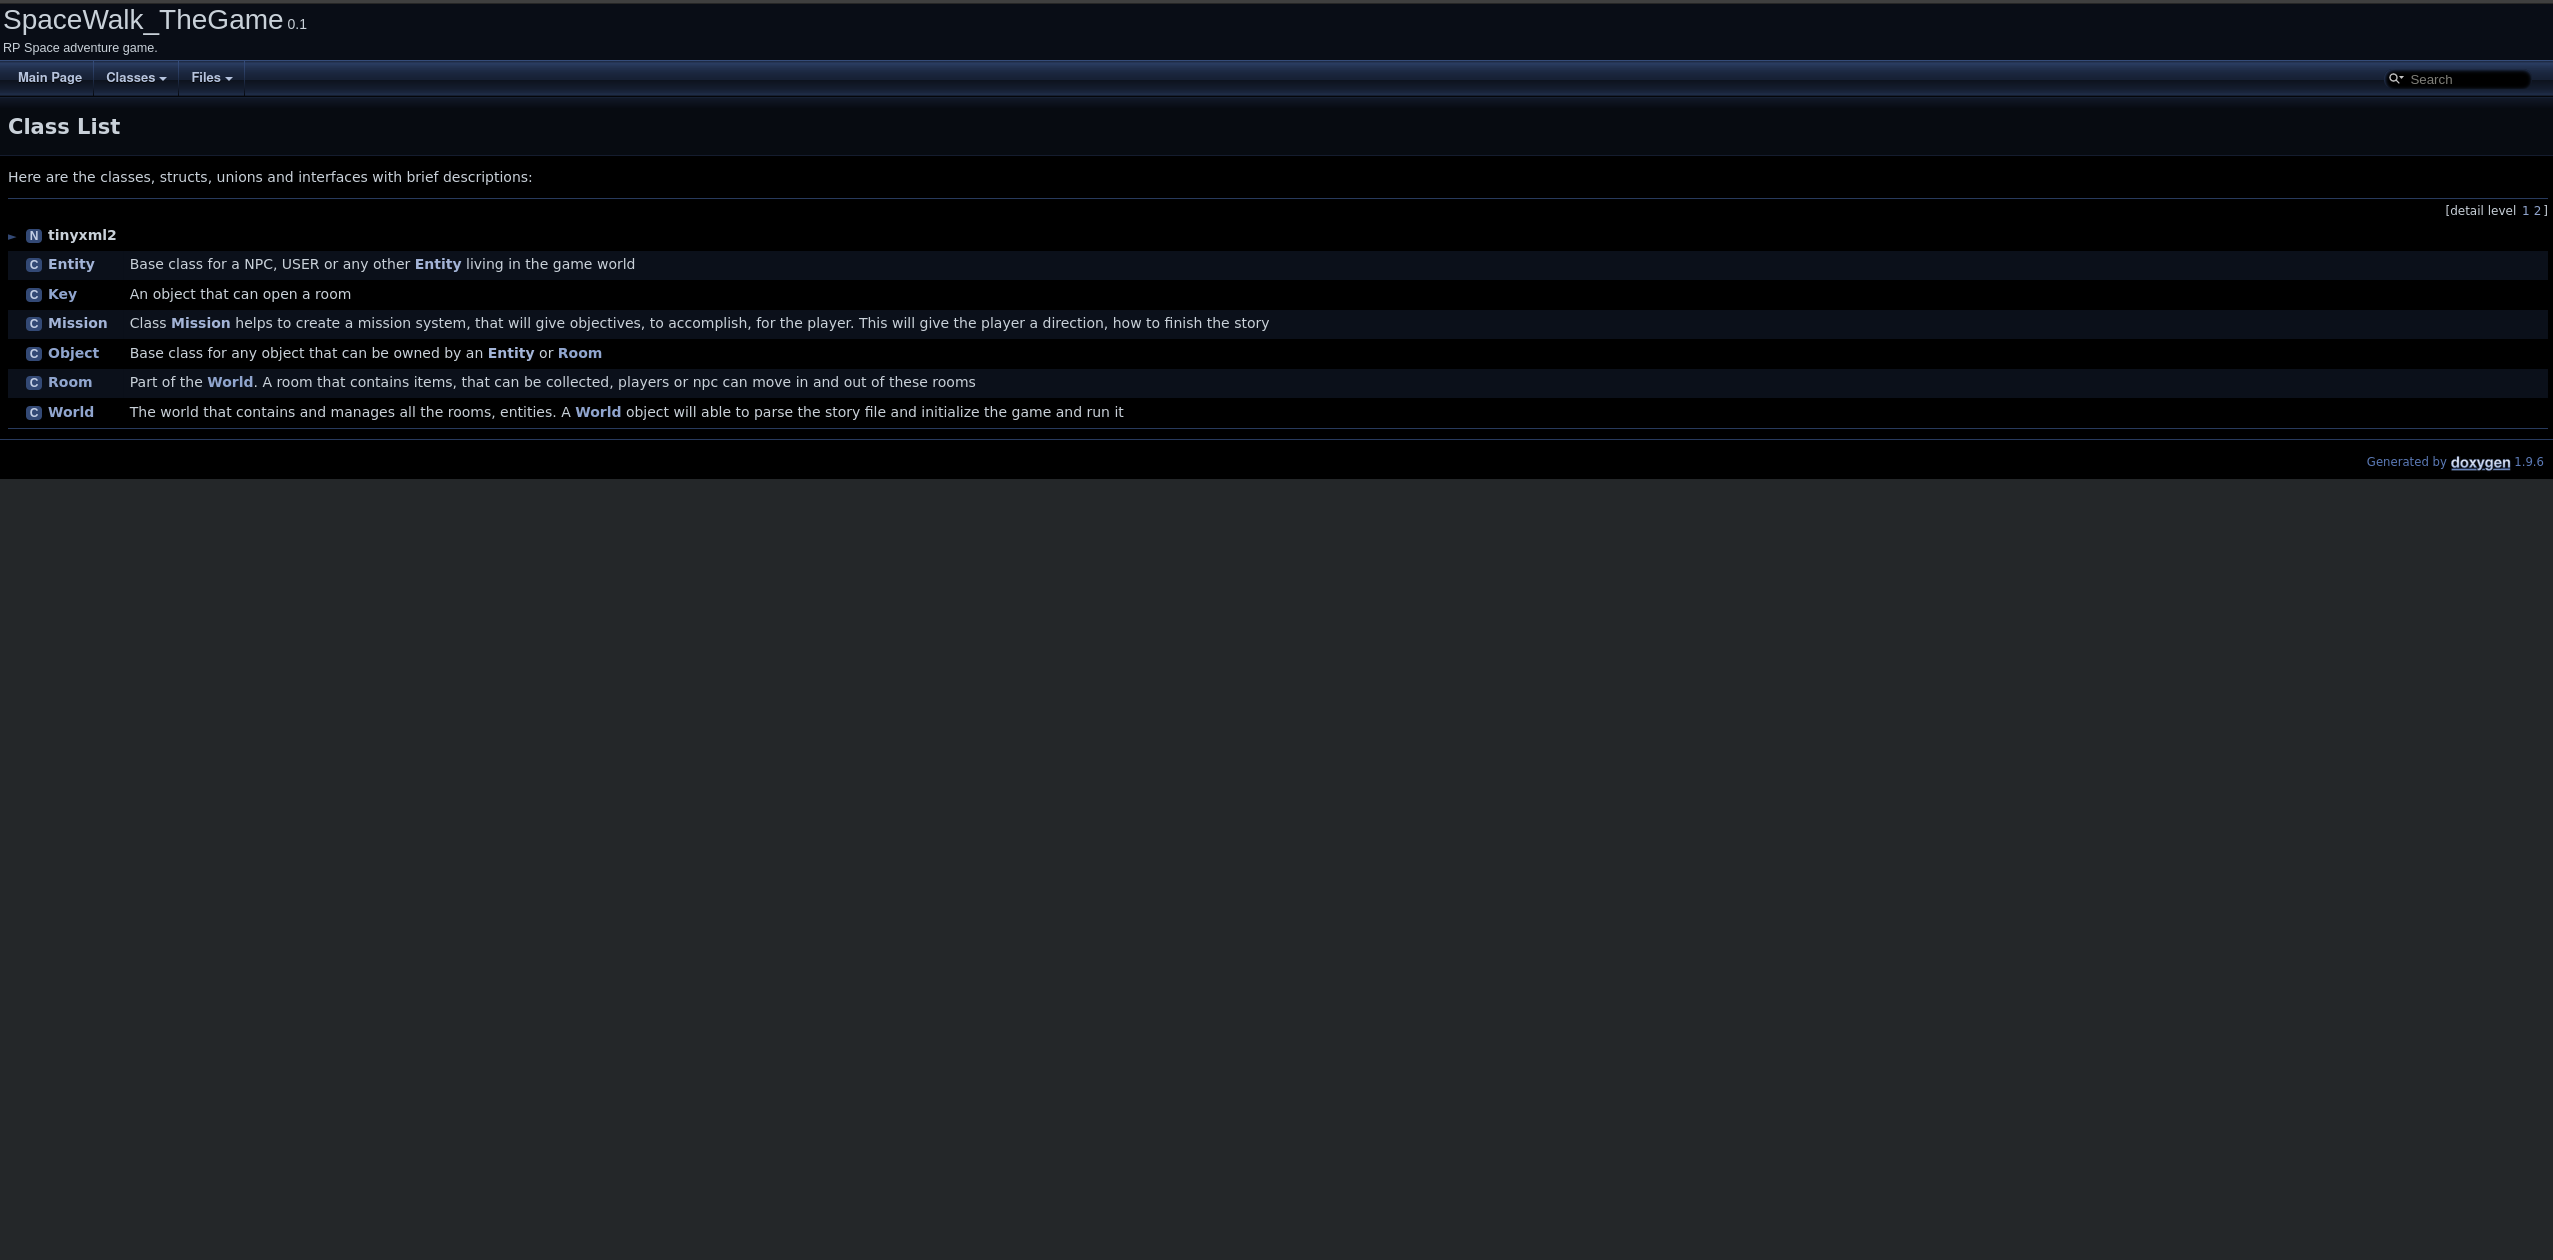
\includegraphics[width=1.0\columnwidth]{doxygen_sample.png}
    \caption{Doxygen}\label{fig:8}
\end{figure}

\section{Fejlesztési eszközök}
\begin{itemize}
    \item Verziókezelés: Git, Szolgáltató: Github
    \item Fejlesztési környezet: VSCode
    \item Fejlesztési környezet kiegészítők: CMake Tools, LaTeX LaTeX Utilites, LaTeX Workshop, Makefile Tools, PlantUML, PlantUMLViewer, Vim, XML Tools
    \item Diagramok elkészítéséhez használt eszközök: VisualParadigm, PlantUML
    \item Operációs rendszerek: Pop! OS (Linux), Windows 10, Windows 11
    \item Dokumentáláshoz használt eszközök: Markdown, LaTeX, Doxygen
    \item Külső könyvtárak: GoogleTest, TinyXML2
    \item Debugger eszközök: GDB, Valgrind
    \item Szövegszerkesztő programok: Word
    \item Kommunikációs platformok: Discord, Messenger
\end{itemize}

\section{Glossary}
\begin{itemize}
    \item Űrkalandjáték: Olyan játék, melynek fő helyszíne a világűr.
    \item Világűr: Az egyes égitestek között jelenlévő légüres tér (vákuum).
    \item Mesterséges intelligencia (Artificial Intelligence - AI): Egy gép, program vagy mesterségesen létrehozott tudat által megnyilvánuló intelligencia.
    \item NPC (Non-Playable Character): Olyan karaktert jelöl a játékban, melyet a játékos nem tud irányítani.
    \item Utópia: Olyan, általában jövőbeli társadalom, mely tökéletes vagy közel tökéletes. (Pl.: Platón - Állam)
    \item Disztópia: Az utópia ellentéte, azaz olyan társadalom, mely szétesőben van vagy az összeomlás felé tart, vagy már el is érte azt. Gyakori témái a háború, az erőszak, az elnyomás és a diktatúra. (Pl.: George Orwell - 1984)
    \item Sci-Fi (Science-Fiction): Olyan alkotás, mely létező vagy kitalált tudományoknak a társadalomra gyakorolt hatását mutatja be.
    \item Jégkorszak: Olyan időszak, amikor az adott égitesten állandó sarki jégtakaró van jelen.
    \item Űrséta: Olyan speciális tevékenység, melynek során az űrhajós teste, vagy testének egy része az űrhajón kívülre kerül.
    \item Aszteroida: 1 méterestől akár 1000 kilométeres átmérőig terjedő, szabálytalan alakú, szilárd anyagú égitest, amely nem rendelkezik atmoszférával, és csillag körül kering.
    \item Szabotázs: Romboló tevékenység, melynek célja valamilyen folyamat késleltetése.
    \item Speifikáció: Részletes ismertető, a tulajdonságok felsorolása és leírása.
    \item Monoton: Egyhangú, változatosság nélküli tevékenység.
    \item Űrállomás: Életfenntartó rendszerrel berendezett bolygó vagy hold körüli pályán keringő űreszköz.
    \item Svédasztal: Ételek felszolgálási módja, mely során egy külön asztalon mutatják be az ételeket és a vendégek igényeiknek megfelelően válogathatnak az asztalról.
    \item Diszkó: Szórakozhely, népszerű zenékkel és tánccal.
    \item Történetvázlat: Rövid, nagy vonalakban történő leírás a történetről és eseményekről. 
    \item Használati eset / use case: Leírja a modellezendő redszer és a környezete kapcsolatát. Célja a követelményrögzítés.
    \item Tesztelés: Olyan folyamat, amely a szoftverfejlesztési életciklushoz kapcsolódik és különböző tevékenységekből tevődik össze. Célja hogy megtalálja a hibákat illetve megnézze, hogy a szotvertermék teljesíti-e a meghatározott követelményeket.
    \item Módszertan: Alkalmazási mód, különböző eljárások és módszerek összessége amelyeket tudatosan felhasználunk a cél elérése érdekében.
    \item XMl: Extensible Markup Language azaz kiterjeszthető jelölőnyelv. Lehetővé teszi egyéni információs formátumok létrehozását és használatát.
    \item TinyXML2: C++ XML-elemző, amely könnyen integrálható más programokba mert egyszerű és hatékony.
    \item GoogleTest: Egy tesztelési keretrendszer, amely platformfüggetlen, nem csak az unit teszteket támogatja, gyors és könnyen tanulható. 
    \item Workflow: Munkafolyamat, egy kitűzött cél elérése érdekében végrehajtott tevékeny-ségek ésszerű sorrendje. 
    \item Scrum: Agilis módszertan szigorú szabályokkal és tág felelősségi körökkel.
    \item Kanban: Emberek csoportos munkájának menedzselésére és fejlesztésére kialakított ütemezési rendszer.
    \item Git: Gráfalapú nyílt forráskódú verziókezelő rendszer.
    \item Github: A Microsoft által üzemeltetett felhőalapú git protokollt használó verziókezelő tárhely. 
    \item VSCode: Ingyenes, nyílt forráskódú kódszerkesztő a modern webes és felhőalapú alkalmazások építéséhez és hibakereséséhez.
    \item Word: A Microsoft által készített dokumetumszerkesztő program.
    \item Discord: Ingyenes VoIP alkalmazás, amely lehetőséget nyújt a felhasználók közötti kommunikációra.
    \item Messenger: Üzenetküldő platform, amit a Facebook fejleszett ki.  
\end{itemize}
\end{document}